\documentclass[11pt,reqno]{amsart}

\usepackage{amsthm,amsmath,amssymb}
\usepackage{mathtools}
\usepackage{proof}
\usepackage{xcolor}
\usepackage{graphicx,wrapfig}
\usepackage[T1]{fontenc}
\usepackage{courier}
\usepackage{hyperref}
\hypersetup{
    hidelinks=true
}
\usepackage{array}
\usepackage{multirow}
\usepackage{listings}
\lstset{basicstyle=\ttfamily\footnotesize, columns=fullflexible, language=C, morekeywords={omp,task,private,pragma,parallel,reduction,single,nowait,num_threads},frame=single, numbers=left}
\newcommand{\code}[1]{\texttt{#1}}
\newcommand\MyBox[2]{
  \fbox{\lower0.75cm
    \vbox to 1.7cm{\vfil
      \hbox to 1.7cm{\hfil\parbox{1.4cm}{#1\\#2}\hfil}
      \vfil}%
  }%
}
\graphicspath{ {./} }

\begin{document}

\begin{center}
\large\textbf{Assignment 1 - Part 2 \\ COMP529 Fall 2019 - Parallel Programming} \\
\normalsize\textbf{Erhan Tezcan 0070881 \\ 03.03.2020} \\
\end{center}

\section{Objective}

We are given an \code{nqueens} solver. The solver basically uses the power of recursion to employ backtracking. We are asked to parallelise this, or more specifically, task parallelise this algorithm. As per request in the assignment file, in this paragraph I state that I have completed all parts.

\section{Design and Implementation}

In my implementation, I have created a task for each recursion in the algorithm. For the outmost level synchronization, I have used \code{taskgroup} directive. Though it is similar to \code{taskwait}, \code{taskwait} only synchronizes to the tasks that were created at that level. \code{taskgroup} on the other hand, synchronizes to the tasks at it's level and their child tasks. So basically, every task created in the group, as well as the tasks created by those tasks, will be finished when we are out of the taskgroup. In other words, we utilize task parallelism, but we do not have any data parallelism. The reason being: each task needs to operate on its own game board. So when each task is created for the recursion, a copy of the game board is also created beforehand and that copy is passed to the task. This of course creates some extra overhead for the creation and copying of the board at each task creation. 

\subsection{Cutoff}

Due to the copious (though not superflous) amount of tasks created, the performance is actually hindered. Considering the number of recursion for a game, there will be many tasks created and that itself is going to be a major overhead. To tackle this problem, a \textit{cutoff} mechanism is used. Notice in the algorithm, we can think of the column number as a depth. The deeper we recurse, the higher columns we have checked. Therefore, it is sensible to construe the column argument as the depth of recursion. Together with a user defined cutoff parameter, beyond some depth the corresponding thread will not create the task, but actually executive that code then and there. We have two alternatives for this conditional task creation: \code{if} and \code{final} clauses. In my implementation, I have used the \code{final} clause. To find the best cutoff parameter, I have conducted a separate experiment, of which I will give more detail about in the next section.

\subsection{Early Termination}

We also test and compare the parallel and serial programs in a case where after the program finds just one solution, it will exit. In both codes, I have used a global variable called \code{terminate} rather than exiting the program at the first solution print. This ``graceful termination'' seemed more sensible and cleaner.

\subsection{Bottlenecks}

In this section let us focus on the bottlenecks in more detail. 
\begin{itemize}
	\item \textbf{Copying the board for each task.} This is a rather big issue because though the board size is small (relative to what would normally be a problematic size) we have a lot of task creations. Each task creation brings a board copy with it, therefore we actually use a lot of memory and spend a significant amount of time on copying the board everytime. Another issue that comes with this is that, the board is \textit{created} at the thread that issues the task, and also copied there. We may see a drop in performance if NUMA comes into play here and the thread that took the task has to give extra effort to obtain that board.
	\item \textbf{Printing the solution.} This is a critical section. If we do not make this a critical section, several threads may want to print their own board at once and therefore cause overlapping prints, which make no sense at the console when we try to read them.
\end{itemize}

\section{Experiments and Evaluation}
We have used \textbf{KUACC} for collecting performance data. The program was compiled with the Intel compiler \code{ICC}. I have used a single batch file for these experiments while using the \code{--exclusive} option for the \code{sbatch} command to make sure it is only me that is using the respective compute node.

\subsection{Executables}
For the following experiments, on some programs I had command line arguments and on some of them I had different executables. Here are the source codes and their executables:
\begin{itemize}
\item \code{nqueens\_serial.c} $\xrightarrow{}$ \code{nqn\_ser}: \\
Serial code given to us.
\item \code{nqueens\_serial-early.c} $\xrightarrow{}$ \code{nqn\_ser\_e}: \\
Serial code with graceful termination upon finding one solution.
\item \code{nqueens\_parallel.c} $\xrightarrow{}$ \code{nqn\_par}: \\ 
Task parallelized version of \code{nqueens\_serial.c}. Has launch option \code{-t} to adjust thread count.
\item \code{nqueens\_parallel\_13.c} $\xrightarrow{}$ \code{nqn\_par\_13}: \\ 
Same as \code{nqueens\_parallel.c} but with board size 13. Has launch option \code{-t} to adjust thread count.
\item \code{nqueens\_parallel\_15.c} $\xrightarrow{}$ \code{nqn\_par\_15}: \\
Same as \code{nqueens\_parallel.c} but with board size 15. Has launch option \code{-t} to adjust thread count.
\item \code{nqueens\_parallel-cutoff.c} $\xrightarrow{}$ \code{nqn\_par\_c}: \\
Modified version of \code{nqueens\_parallel.c} with cutoff functionality where it does not create tasks after some depth of recursion. Has launch option \code{-t} to adjust thread count and \code{-c} to adjust cutoff parameter.
\item \code{nqueens\_parallel-early.c} $\xrightarrow{}$ \code{nqn\_par\_e}: \\
Modified version of \code{nqueens\_parallel.c} that gracefully terminates upon finding one solution. Has launch option \code{-t} to adjust thread count.
\end{itemize}

I have also included a compilation script so that it is easy to compile these programs all at once if needed, I will be including this script in the submission.
\subsection{Cutoff Parameter}

We would like to know which cutoff parameter is best performing, therefore we conducted another experiment (\code{cutoff.sh} is the job script for that) and we obtained the figures \ref{fig:cutoff_exp_c} and \ref{fig:cutoff_exp_s}.

\begin{figure}[h]
\centering
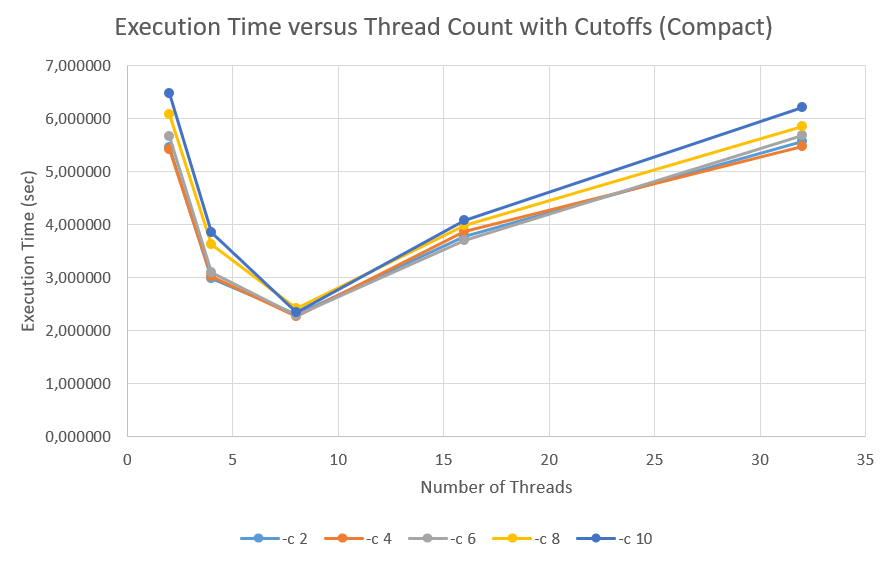
\includegraphics[width=0.75\linewidth]{cutoff_compare_compact.png}
\caption{Execution Time versus Thread Count with Cutoff on Compact affinity.}
\label{fig:cutoff_exp_c}
\end{figure}

\begin{figure}[h]
\centering
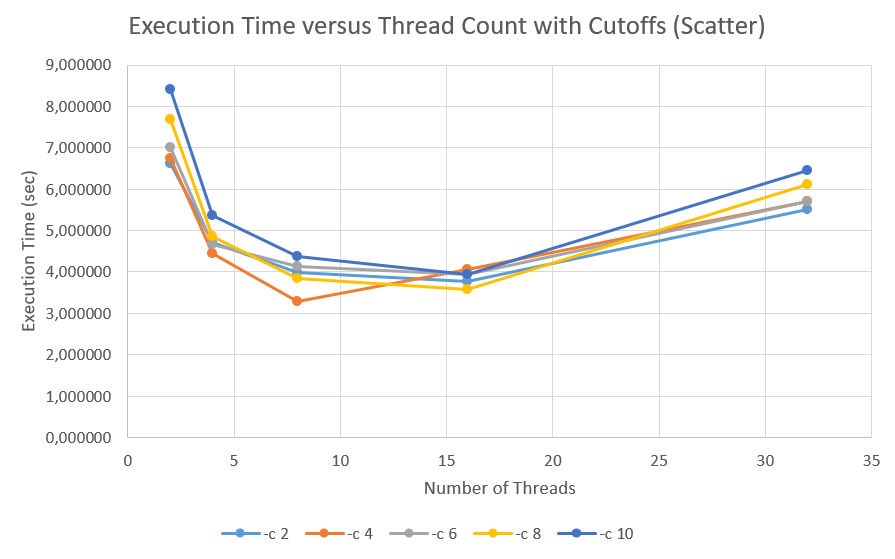
\includegraphics[width=0.75\linewidth]{cutoff_compare_scatter.png}
\caption{Execution Time versus Thread Count with Cutoff on Scatter affinity.}
\label{fig:cutoff_exp_s}
\end{figure}

From these graphs, we concluded that 4 and 6 are performing really well, with 4 performing way better for the scatter affinity scenario. For the best of both worlds, we have decided to use cutoff parameter of 5. This means that after the 5th column of the board, there will not be task creations, but rather they will be executed right there.

\subsection{\code{KMP\_AFFINITY} Compact}
In this section, we will be evaluating the experiments done with the \code{KMP\_AFFINITY} environment variable set to \code{granularity=fine,compact}. 

\subsubsection{Part-II-A and Part-II-B}
We would like to show the results of both experiments on the same graph since that makes it more clear how the performance is achieved.

\begin{figure}[h]
\centering
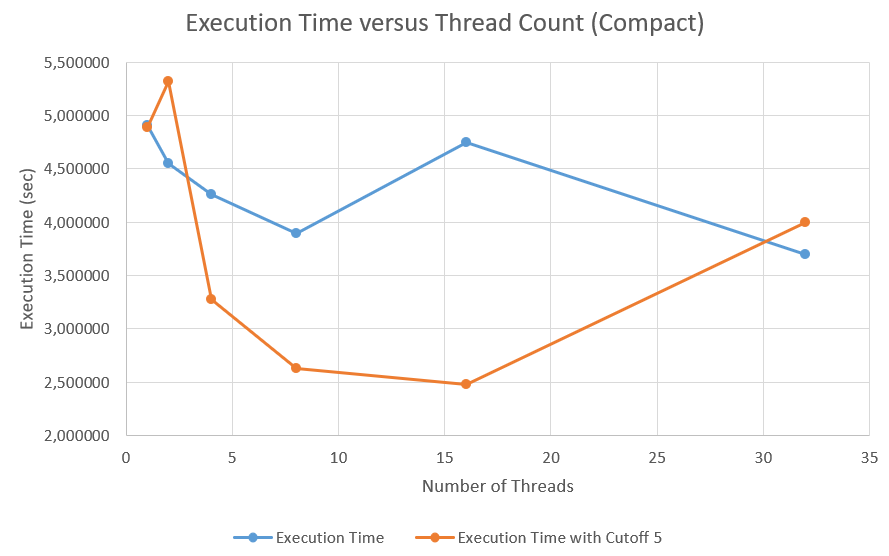
\includegraphics[width=0.75\linewidth]{exectime_A_B_compact.png}
\caption{Execution Time versus Thread Count.}
\label{fig:exec_A_B_c}
\end{figure}

\begin{figure}[h]
\centering
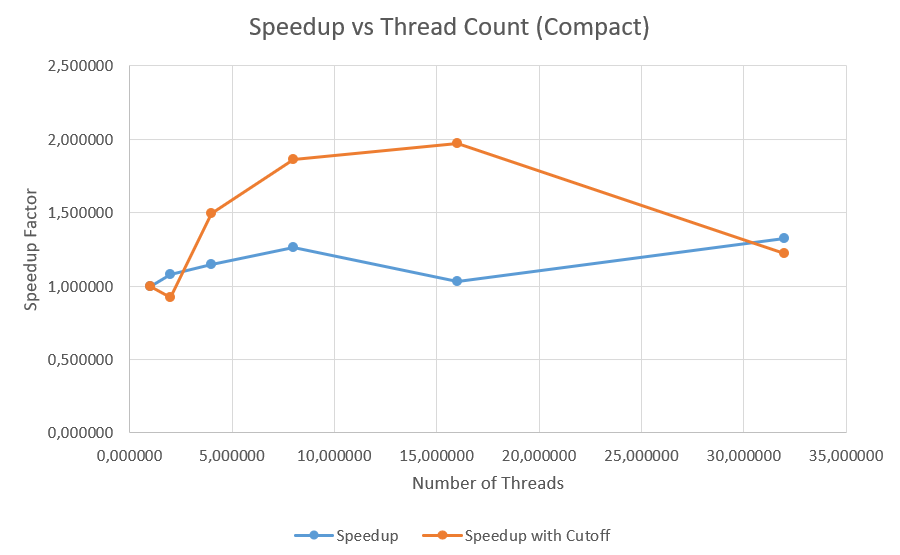
\includegraphics[width=0.75\linewidth]{speedup_A_B_compact.png}
\caption{Speedup versus Thread Count.}
\label{fig:spd_A_B_c}
\end{figure}

In figure \ref{fig:exec_A_B_c} we observe immediately that we have slightly good performance but it is not really what we would expect. The reason being is that the amount of tasks are huge and there are too many ``shopping'' of tasks, in other words, threads are constantly taking a task, finishing it, taking another task and so on. With this many tasks, regardless of how many threads we have the performance will not be that good. By introducing cutoff, we are able to observe the expected scaling. We can see the performance gain more clearly wen we look at the speedup graph on figure \ref{fig:spd_A_B_c}. We have increasing speedup as we go from 2 threads to 16, but at 32 threads we observe drop in speedup. It is still faster than the serial, but the reason of the drop of performance with 32 threads is the fact that our machine may not have 32 processing units available. If the machine has 16 processing units and we issue 32 thread directives this will cause drop of performance, also because it introduces more overhead and more memory latencies.

\subsubsection{Part-II-C}

\begin{figure}[h]
\centering
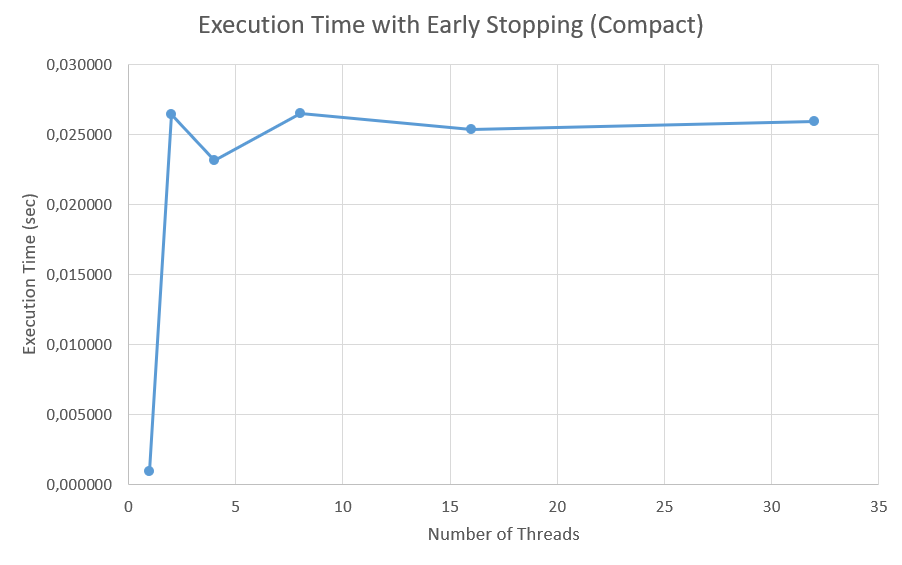
\includegraphics[width=0.75\linewidth]{early_stop_compact.png}
\caption{Execution Time versus Thread Count.}
\label{fig:early_c}
\end{figure}

\begin{figure}[h]
\centering
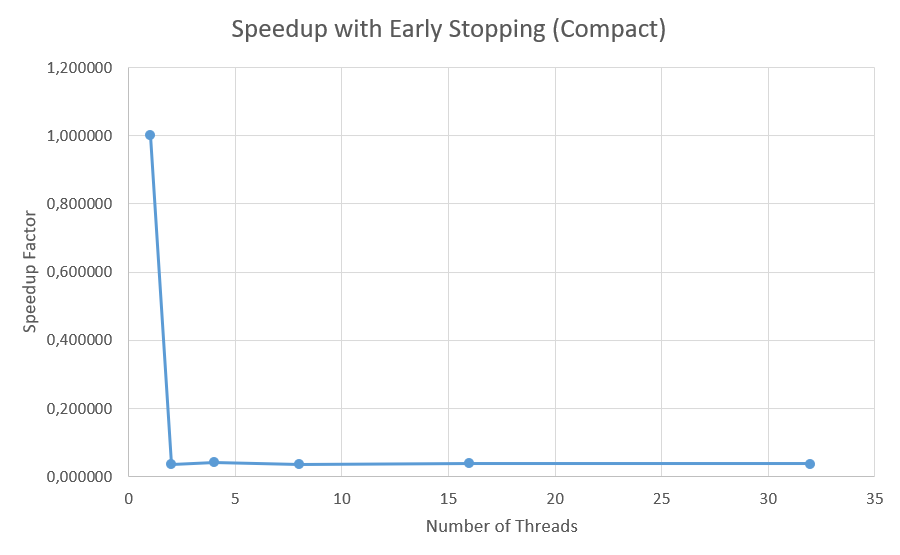
\includegraphics[width=0.75\linewidth]{speed_early_stop_compact.png}
\caption{Speedup versus Thread Count.}
\label{fig:speed_early_c}
\end{figure}

In the early stopping cases (figures \ref{fig:early_c} and \ref{fig:speed_early_c}) we see that serial code is way faster than the parallel code! Again, here the thread launch and task launch overheads play an important role. If we imagine the possible boards in a tree structure, where the root is an empty board, the serial code is searching for the solution in a depth first manner. The parallel code however, is doing both breadth first and depth first search. How is it doing that? Well, the tasks are launched in a breadth first manner, and each task is operating on a deeper level. By the nature of the problem, we know that the solution exists at the deepest layer when we think of the layers as columns. So a depth first search would win for sure, compared to both breadth first and depth first search. We might still ask, the parallel program is also doing depth first search in itself, so why is it still slow? That is because the overhead and computation of managing so many tasks and threads is hindering the performance.

\subsubsection{Problem Sizes Comparison}

In figure \ref{fig:size_c} we can see how the execution time scales with the problem size. Expectedly, it is rising. Intuitively, we would expect the amount of effort to find a single solution should be similar. To prove this, we also added another result to the graph, shown as dashed line, where we divide the number of solution to the execution time. To show these in a single graph, we also multiply that number by $10^{-4}$ and we can see that it's value is similar for 13, 14 and 15 board size cases.

\begin{figure}[h]
\centering
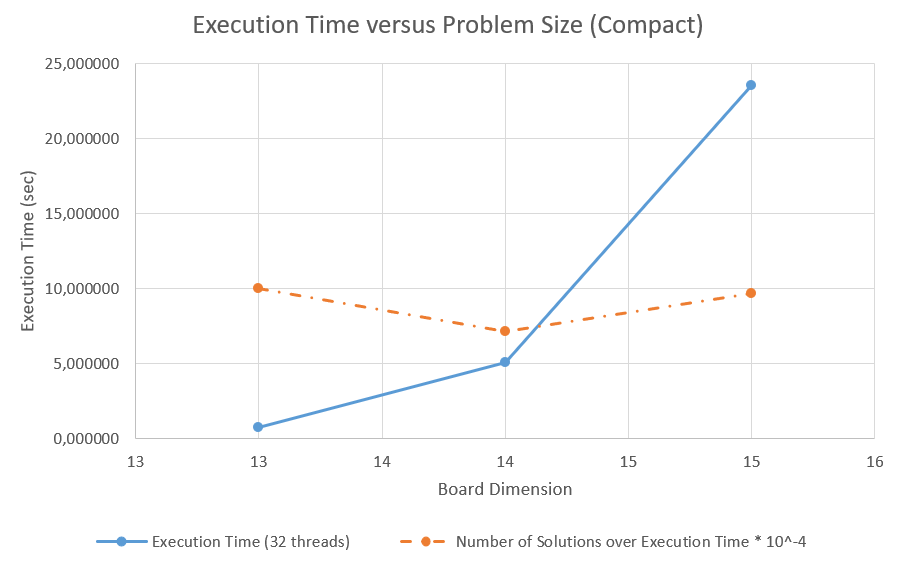
\includegraphics[width=0.75\linewidth]{problem_size_compact.png}
\caption{Execution Time versus Problem Size.}
\label{fig:size_c}
\end{figure}

\subsection{\code{KMP\_AFFINITY} Scatter}
In this section, we will be evaluating the experiments done with the \code{KMP\_AFFINITY} environment variable set to \code{granularity=fine,scatter}. 

\subsubsection{Part-II-A and Part-II-B}
Again, we would like to show the results of both experiments on the same graph (figures \ref{fig:exec_A_B_s} and \ref{fig:spd_A_B_s}) since that makes it more clear how the performance is achieved. Just looking at this alone we can see that with scatter affinit we do not have much performance gain, regardless of the cutoff mechanism. We do however observe a bit of speedup at 4 threads, but for the remaining thread counts it stays rather constant. Of course, with cutoff the program runs slightly faster.

The reason behind these figures could be perhaps because when a thread takes on the task, it will create another task almost immediately, but in doing so it will create a copy of the board itself. Then the thread that will take this newly created task will also need that board, thus if these two threads resided close to each other that would be better. In compact case, this is more likely to happen compared to scatter case, where the threads are basically scattered across the processors. This is also perhaps why we do not see here the drop of performance at 32 threads like we observed at compact affinity.

\begin{figure}[h]
\centering
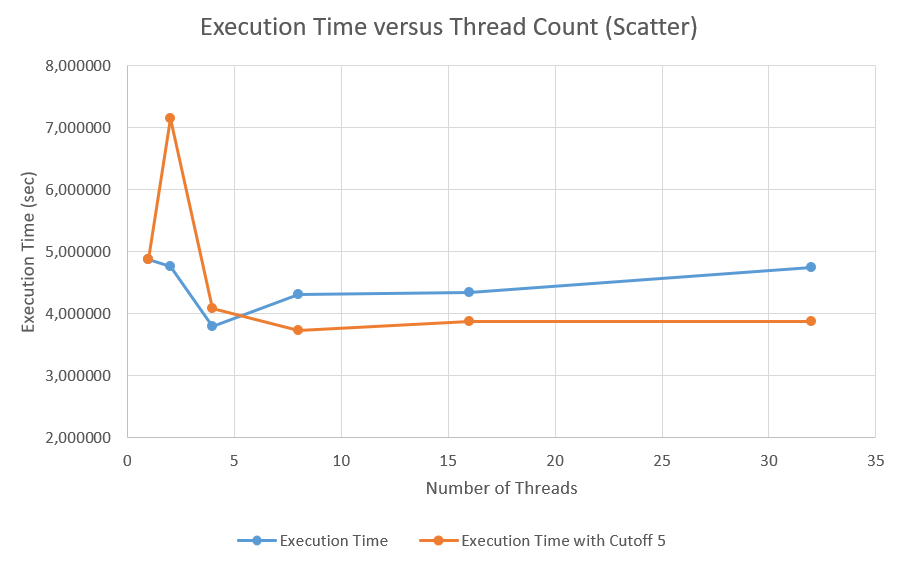
\includegraphics[width=0.75\linewidth]{exectime_A_B_scatter.png}
\caption{Execution Time versus Thread Count.}
\label{fig:exec_A_B_s}
\end{figure}

\begin{figure}[h]
\centering
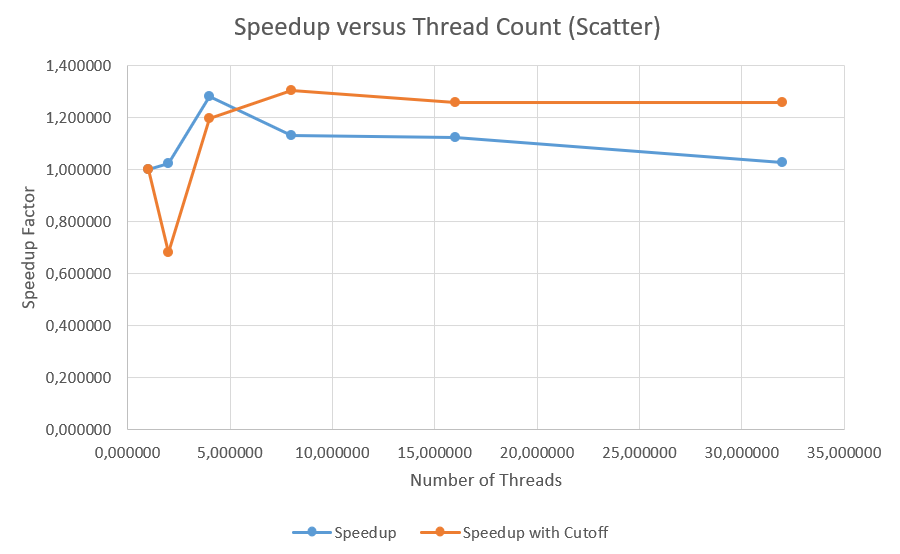
\includegraphics[width=0.75\linewidth]{speedup_A_B_scatter.png}
\caption{Speedup versus Thread Count.}
\label{fig:spd_A_B_s}
\end{figure}

\newpage

\subsubsection{Part-II-C}
In figures \ref{fig:early_s} and \ref{fig:speed_early_s}, again we observe that the single case is way faster than the parallel case. The reasons are same as discussed in the section with this experiment for the compact affinity.
\begin{figure}[h]
\centering
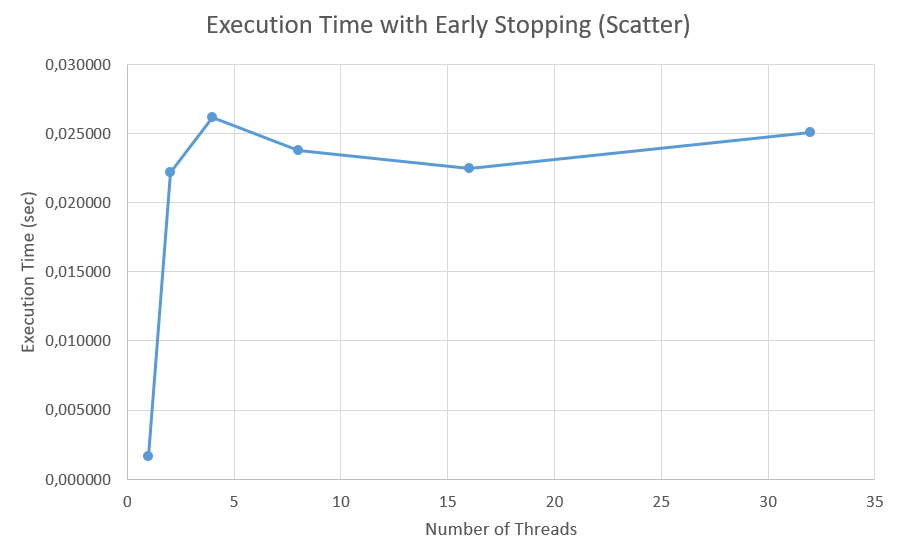
\includegraphics[width=0.75\linewidth]{early_stop_scatter.png}
\caption{Execution Time versus Thread Count.}
\label{fig:early_s}
\end{figure}

\begin{figure}[h]
\centering
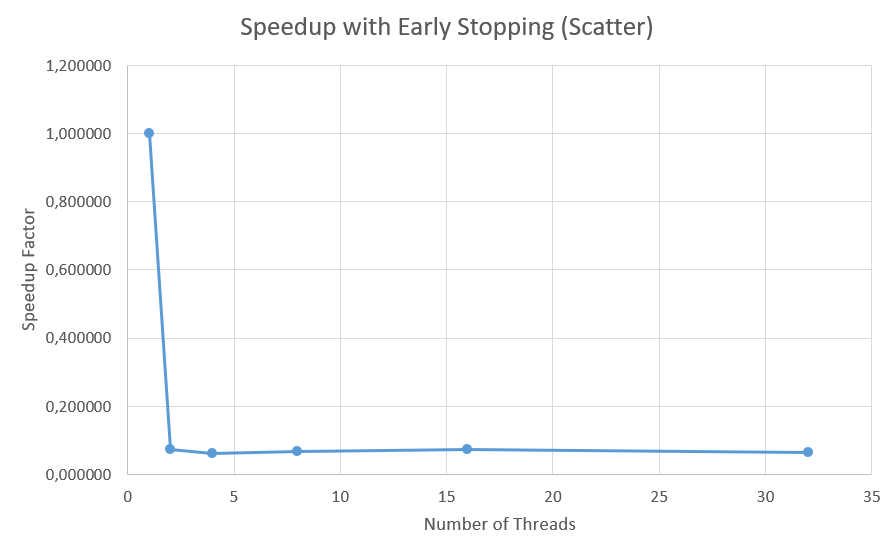
\includegraphics[width=0.75\linewidth]{speed_early_stop_scatter.png}
\caption{Speedup versus Thread Count.}
\label{fig:speed_early_s}
\end{figure}

\subsubsection{Problem Sizes Comparison}

We see a similar scaling of the execution time as the board dimension gets bigger, and as we have mentioned before we draw an extra line where we divide the number of solutions to the execution time, and observe that it is almost constant. So this experiment is also resulting in a similar fashion with compact affinity.
\begin{figure}[h]
\centering
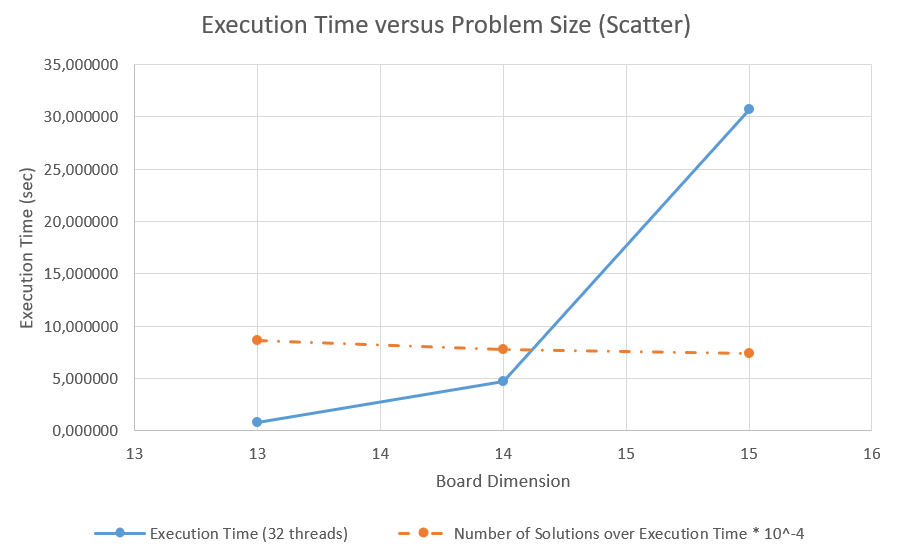
\includegraphics[width=0.75\linewidth]{problem_size_scatter.png}
\caption{Execution Time versus Problem Size.}
\label{fig:size_s}
\end{figure}

\section{Conclusion}
To conclude, we have observed that by utilising task parallelism we can achieve performance on the \code{nqueens} problem. However, the thread affinity plays an important role on the scalability of the program. This affinity should also be thought with the nature of the problem in mind (recall that we mention depth first and breadth first search) and should be chosen accordingly. We also observed that a single solution search works better if we use the serial program, mostly because that way we are able to avoid the immense overheads of thread and task creations. 
We have also seen that on a machine with 16 processing units, 32 threads will perform worse. This is becuase the machine simply does not have that many processing units but it will obey with the OpenMP's rules. As a result, there will be a lot of thread's taking place of each other and consequently lots of memory latency and cache coherency problems.
\end{document}